


\chapter{Introduction}\hrule
\label{Chapter:1}
% =====================================================================================================
\section{Introduction to project}

Sentiment is an attitude, thought, or judgment prompted by feeling. Sentiment analysis [1-8], which is also known as opinion mining, studies people’s sentiments towards certain entities. Internet is a resourceful place with respect to sentiment information. From a user’s perspective, people are able to post their own content through various social media, such as forums, micro-blogs, or online social networking sites. From a researcher’s perspective, many social media sites release their application programming interfaces (APIs), prompting data collection and analysis by researchers and developers.\\
\\
 For instance, Twitter currently has three different versions of APIs available [9], namely the REST API, the Search API, and the Streaming API. With the REST API, developers are able to gather status data and user information; the Search API allows developers to query specific Twitter content, whereas the Streaming API is able to collect Twitter content in realtime. Moreover, developers can mix those APIs to create their own applications. Hence, sentiment analysis seems having a strong fundament with the support of massive online data.\\
What is Sentiment?\\ 
Sentiment = feelings\\
1.Attitudes\\
2.Emotions\\
3.Opinions\\

Usually reviews are given in text format. Single product has number of reviews. It is hardly
possible to read each review in detail. Many researches shown pictorial representation is more
effective and can be memorized, understood easily rather than textual representations. So if we
are going to convert textual reviews into visual format, it will enhance reliability in decision making.

\section{Project Category}
This project is categorized System Development. This project is a product review System, which analyse the product reviews and shows out the sentiment in chart forms. It gives us detailed examination of the product reviews.

\section{Objectives} 

Sentiment analysis or opinion mining is a field of study that analyzes people’s sentiments, attitudes, or emotions towards certain entities. This paper tackles a fundamental problem of sentiment analysis, sentiment polarity categorization. \\
1. Online product reviews any website can be selected as data used for this study.\\
2.A sentiment polarity categorization process  has been proposed along with detailed description of each step.\\
3.Experiments for both sentence-level categorization and review-level categorization have been performed.\\

\section{Problem Formulation}
“What other people think” has always been an important piece of information for most of us during the decision-making process. The product makers need to analyze the reviews of the product for planning and executing the future projects.

\section{Recognition of Needs}
After launching a product, the company needs to analyze the review of the product. Going through each and every product review can become very exhaustive. Thus we need such a system which interactively shows the sentiments of product reviews using graphs, so that we can save our time and efforts.

\section{Existing System}

Existing work shows that various approaches are used for Sentiment Analysis like machine
learning, corpus based, NLP based or even based on clustering. Also few researches consider
neutral review for analysis. Many of them do not have visual representations for end results or
complex visual representations which are not user oriented.

\section{Proposed System}
While doing analysis of product reviews, company needs to know:
\begin{itemize}
	\item Does the product has satisfied a big pool of customers?
	\item Are the customer reviews positive or negative?
	\item Analyze each individual's reviews
    \item Finally producing the overview of analyzed results.
\end{itemize}

Thus keeping these points a system should be developed which represents product reviews in a better way.

\section{Unique features of the System}
\begin{itemize}
	\item Unsupervised Machine learning i.e Machine trains itself on the available data to the machine.
	\item Analyzing the comment using words, then sentences, then whole paragraph and then giving the over all result.
	\item Showing the results of the analyzed data.
	\item Plotting the pie chart of analyzed data.
\end{itemize}




\chapter{Requirement Analysis and System Specification }\hrule
\label{Chapter:2}
% =====================================================================================================

\section{Feasibility Study}
In feasibility study phase we had undergone through various steps:\\
1.\textbf{Technical Feasibility} : This project Sentiment Intelligence will be platform independent. It
is coded in Python. Hardware requirements used are compatible with all OS. The system can also be expanded as per the needs of requirement specification.\\
2.\textbf{Economic Feasibility}: The cost required in the proposed system is economic and
affordable as no additional hardware is required for the project. We need only manpower
i.e skilled person who knows python and has worked on various python libraries like
SCIKIT-LEARN, NLTK, BEAUTIFULSOUP etc.\\
3.\textbf{Legal Feasibility}: Since this application involves no specific society membership, it is
totally feasible legally. It the proposed system conflicts with legal requirements like data
protection acts or social media laws.\\
4.\textbf{Operational Feasibility}: As per requirement, the proposed solution will provide a tool to
the various film production companies to analyze their business needs and customer review for their project.
5.\textbf{ Scheduling Feasibility}: The project is estimated to complete within a time span of 60
working days. 24 days for SRS documentation, 24 days for product design and code, 12
days for unit and integration testing.

\section{Software Requirement Specification}

\subsection{\textbf{Introduction}}

\subsubsection{Purpose}
\begin{itemize}
	\item To develop an easier system for review analysis of a product
	\item Clear and Concise results available after analysis
	\item Business oriented results
	\item Results can be used for enhancing the upcoming products on the basis of already launched product review.  
\end{itemize}

\subsubsection{Scope}
\begin{itemize}
	\item Product has a brighter future. It can be used as a review analysis system for any product launched by any company.
	\item Artificial Intelligence can be further used in the product to automate it to a particular type of inputs.
\end{itemize}

\subsection{General Requirements}

\subsubsection{Project Perspective}
We need people who have knowledge and hands on experience on python and data science libraries like nltk, beautifulsoup, numpy etc. We also need personal systems for every team member with python installed on it and having at least 2gb Ram installed on the system. 

\subsubsection{Product Function}
Product will provide a system to take input of the product user and will analyze its positivity or negativity of the comment. 

\subsubsection{Constraints}
Product needs a csv file as input. So, you need to convert user comments into .csv format to analyze the data generated by the user. 

\subsection{Specific Requirement}
\begin{itemize}
	\item Need a .csv format input.
	\item Need permission of accessing the survey website legally.
	\item Need a working Internet connection. 
	\item Need specific manpower who have knowledge of python.
\end{itemize}

\subsection{Project Development Plan}
\subsubsection{Purpose}
Produce an Analyzer System to :
\begin{itemize}
	\item Take user inputs as .csv
	\item To show positivity and negativity of the comment
\end{itemize}

\subsubsection{Team Members}
\begin{itemize}
	\item \textbf {Nikant: } Programmer and Team Lead
	\item \textbf {Amulya Garg: } Programmer and planner
	\item \textbf{Prabhudeep Singh: } Programmer and Milestone writer
\end{itemize}

\subsubsection{Timeline}
Days 0-15 -- Requirement Specifications \\
Days 15-22 -- Design Prototype\\
Days 22-25 -- Module Design\\
Days 25-50 -- Coding\\
Days 50-65 -- Analyzing the data \\
Days 65-70 -- Generating the results \\
Days 75-80 -- Publishing the results \\
Days 80-90 -- Unit and Integration Testing \\ 
Day  90    -- Project Fininshed

\section{Expected Hurdles}
\begin{itemize}
	\item Training Machine to generate bag of words 
	\item Fetching output in .csv format
	\item Plotting Charts
\end{itemize}

\section{SDLC Model: Rapid Application Development (RAD)}
\subsection{Introduction to RAD}
RAD model is Rapid Application Development model. It is a type of incremental model. In RAD model the components or functions are developed in parallel as if they were mini projects. The developments are time boxed, delivered and then assembled into a working prototype.  This can quickly give the customer something to see and use and to provide feedback regarding the delivery and their requirements.

\subsection{Advantages of RAD}
\begin{itemize}
	\item Reduced development time.
	\item Increases reusability of components
	\item Quick initial reviews occur
	\item Encourages customer feedback
	\item Integration from very beginning solves a lot of integration issues.
	
\end{itemize}

\subsection{Why RAD Model?}
\begin{itemize}
	\item RAD should be used when there is a need to create a system that can be modularized in 2-3 months of time.
	
	\item It should be used if there’s high availability of designers for modeling and the budget is high enough to afford their cost along with the cost of automated code generating tools.
	
	\item RAD SDLC model should be chosen only if resources with high business knowledge are available and there is a need to produce the system in a short span of time (2-3 months).
\end{itemize}

\chapter{System Design}\hrule
\label{Chapter:3}
% =====================================================================================================

\section{Design Approach}
Design Approach for this system is Object Oriented. The key ideas of the object oriented approach are :

\begin{itemize}
	\item Objects
	\item Encapsulation
	\item Class and Inheritance
	\item Instances and Instantiation
	\item Methods and Messages
\end{itemize}

On of the main principles in the object oriented (OO) approach is that of abstraction, not of data structures and processes separately but both together. An object is a set of data structures and the methods or operations needed to access those structures.

Encapsulation of data structures and methods means that only the methods associated with the object can access the internal data structures. An object is a packaged item of information including the processes which manipulate it. Although we saw above that it is possible to create such packages in e.g. C, the language did not specifically support or enforce the encapsulation.

The objects in OO software are reusable components which may often be used in different applications. In OO environments, object libraries may be available for the programmer to build into solutions.

Generic objects representing classes can also be defined and objects representing subclasses can inherit the data structures and methods from the broader classes to which they belong. A particular instance of a class is represented by instantiating the data structure to the appropriate values.

A programmer may define the structure of an object to represent person and then a new object for employee. The employee object will inherit the data structures and methods from the person object. Note that this inheritance property is equivalent to the is a relation in semantic nets.

\section{Detail Design}

\subsection{Input}
The input to the system is a .csv file, in which different polarities of different id's are defined. A .csv file is a comma seperated values integrated in a single file.

\subsection{Machine Learning}
Machine learning is a type of artificial intelligence (AI) that provides computers with the ability to learn without being explicitly programmed. Machine learning focuses on the development of computer programs that can change when exposed to new data.

The process of machine learning is similar to that of data mining. Both systems search through data to look for patterns. However, instead of extracting data for human comprehension -- as is the case in data mining applications -- machine learning uses that data to detect patterns in data and adjust program actions accordingly.  Machine learning algorithms are often categorized as being supervised or unsupervized. Supervised algorithms can apply what has been learned in the past to new data. Unsupervised algorithms can draw inferences from datasets.

\subsection{Machine review analysis}

After Machine learning is completed, the machine analys and gives Machine analysis review. The generated Machine analysis review from bag of words is further written in a .csv format. Now this .csv file is used to give visualised results of the analysis.

\section{Flowchart }
\begin{figure}[h]
	\centering
	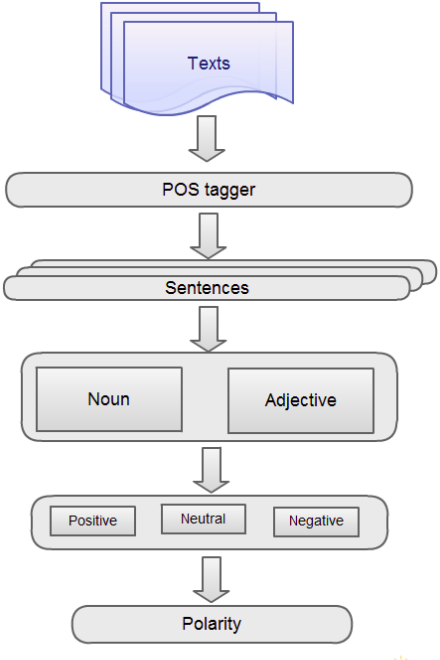
\includegraphics[width=0.7\linewidth]{flow}
	\caption{Flow Chart demonstrating the project}
\end{figure}

\section{Methodology}

\subsection{Data Preprocessing }
Data Preprocessing includes proper fragmentation of data and leaning of data. Here, in research work we are going to use NLP preprocessing techniques like removal of stop words, chunking data, stemming etc. Data preprocessing will lead us to robust data which has less moice. For data preprocessing, use of NLTK library implemented in python is considered. NLTK is a platform for natural language processing developed in python.

\subsection{POS tagging}
POS tagging assists us to identify actual part of sentence which has expression or feelings. It deals with Word Sense Disambiguity(WSD). Single word may have one or more tags. Thus, POS tagging is used to determine single tag for instance of word.
\subsection{Text Classification}
The process of text classification is divided into two stages: Training stage and Testing stage. In training stage, classification model is created using testing dataset. In testing stage, accuracy of classification is evaluated using classification module.
\chapter{Implementation, Testing and Maintanence}\hrule
\label{Chapter:4}
% =====================================================================================================

\section{Introduction to language}

In the back end,Python is used. Concepts and libraries related to data science and deep learning are used. Python is one of the world's most important and widely used computer languages, and it has held this distinction for many years. Unlike some other computer languages whose influence has weared with passage of time, while Python has grown.

As of 2017, Python is one of the most popular programming languages in use, particularly for data science applications, with a reported 11 million developers using and working on it.

\textbf{Applications of Python:}\\
Python is widely used in every corner of world and of human life. Python is not only used in softwares but is also widely used in designing hardware controlling software components. There are more than 100 million python development tool downloads each year.

Following are some other usage of Python :
\begin{itemize}
	\item Web Applications like Linkedin.com, Snapdeal.com etc.
	\item	Cross platform Mobile application development.
	\item Internet of things is widely using it.
	\item	Embedded Systems.
	\item Robotics and games etc.
\end{itemize}

\textbf{Supporting Languages}\\
Follwing Libraries are used:
\begin{itemize}
	\item NLTK(natural language processing toolkit).
	\item Gensim.
	\item Scipy.
	\item bs4.
	\item Pandas.
\end{itemize}
Along with these Libraries, some inbuilt methods of python development kit are also used.\\

\section{Coding Standards}
\begin{itemize}
	\item Use single quotes
	\item Imports
	\item camelCase
	\item PascalCase
	\item PEP 257 (Docstring Conventions)
	\item Referencing other code objects with :py:\\
	\\
	\\
	\\

	
	
\end{itemize}
\section{Project Scheduling}
\subsection{PERT chart}
\begin{figure}[h]
	\centering
	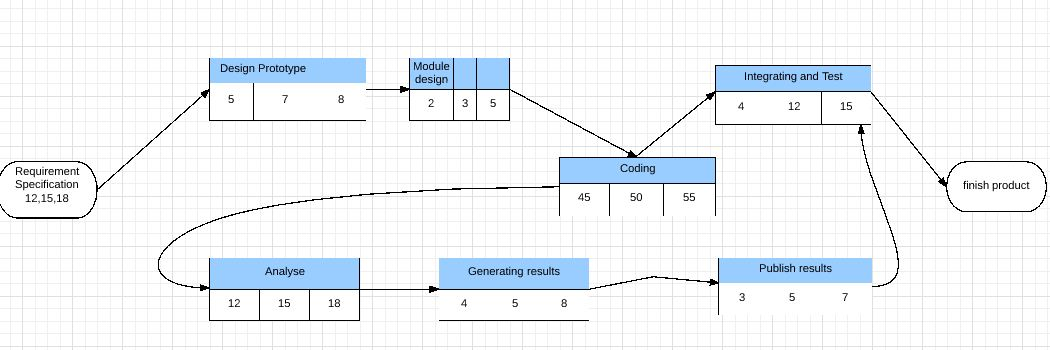
\includegraphics[width=1\linewidth]{pert_final}
	\caption{Pert Chart for project Scheduling}
\end{figure}
A PERT chart is a project management tool used to schedule, organize, and coordinate tasks within a project. PERT stands for Program Evaluation Review Technique, a methodology developed by the U.S. Navy in the 1950s to manage the Polaris submarine missile program.\\
A PERT chart presents a graphic illustration of a project as a network diagram consisting of numbered nodes (either circles or rectangles) representing events, or milestones in the project linked by labelled vectors (directional lines) representing tasks in the project. The direction of the arrows on the lines indicates the sequence of tasks.\\
The PERT chart is sometimes preferred over the Gantt chart, another popular project management charting method, because it clearly illustrates task dependencies. On the other hand, the PERT chart can be much more difficult to interpret, especially on complex projects.

\chapter{Results and Discussions}\hrule
\label{Chapter:5}
% =====================================================================================================
\section{Various Modules of the System}

\subsection{Input}
The input to the system is a .csv file, in which different polarities of different id's are defined. A .csv file is a comma seperated values integrated in a single file.

\subsection{Machine Learning}
Machine learning is a type of artificial intelligence (AI) that provides computers with the ability to learn without being explicitly programmed. Machine learning focuses on the development of computer programs that can change when exposed to new data.

The process of machine learning is similar to that of data mining. Both systems search through data to look for patterns. However, instead of extracting data for human comprehension -- as is the case in data mining applications -- machine learning uses that data to detect patterns in data and adjust program actions accordingly.  Machine learning algorithms are often categorized as being supervised or unsupervized. Supervised algorithms can apply what has been learned in the past to new data. Unsupervised algorithms can draw inferences from datasets.

\subsection{Machine review analysis}

After Machine learning is completed, the machine analys and gives Machine analysis review. The generated Machine analysis review from bag of words is further written in a .csv format. Now this .csv file is used to give visualised results of the analysis.
\section{Snapshots of System}
\begin{figure}[h]
	\centering
	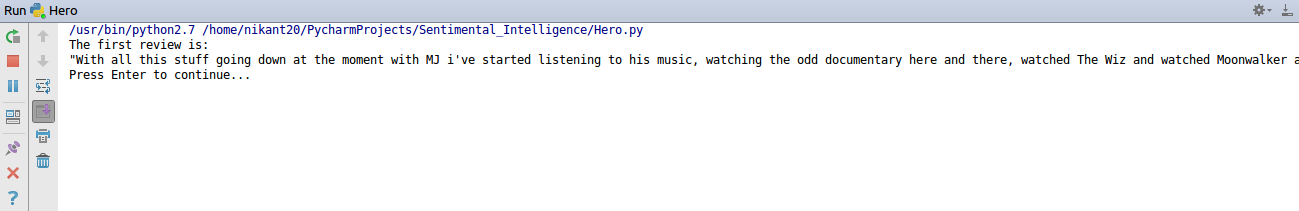
\includegraphics[width=1\linewidth]{1st}
	\caption{Fetching the review}
	\end{figure}
In this picture, the reviews from the .csv file is being fetched and is getting ready to be trained.\\
\begin{figure}[h]
	\centering
	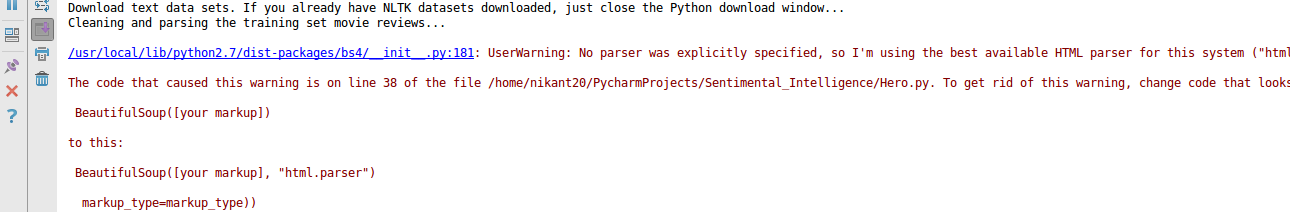
\includegraphics[width=1\linewidth]{2nd}
	\caption{Downloading the NLTK library}
\end{figure}

In this, Python downloads the data associated with the NLTK library. If it is already available, then it uses that available data.\\
\begin{figure}[h]
	\centering
	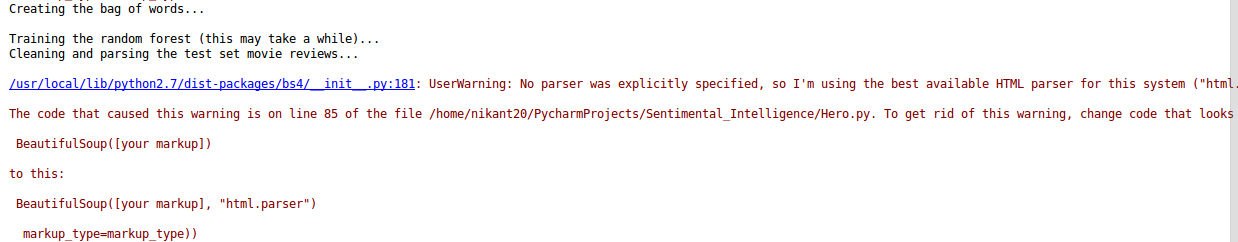
\includegraphics[width=1\linewidth]{3rd}
	\caption{Training the Machine to learn from data}
\end{figure} 

In this, Machine is training itself on the random data from .csv file using random forest algorithm.
\begin{figure}[h]
	\centering
	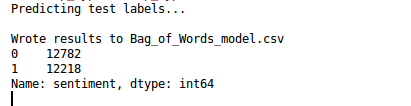
\includegraphics[width=1\linewidth]{4th}
	\caption{Displaying the results after analyzing the .csv file}
\end{figure}

In this, after learning from the data, the machine has analyzed the sample data and has predicted the number of Positive and Negative reviews available in the data. Where 0 stands for Negative value and 1 stands for Positive value.\\
\begin{figure}[h]
	\centering
	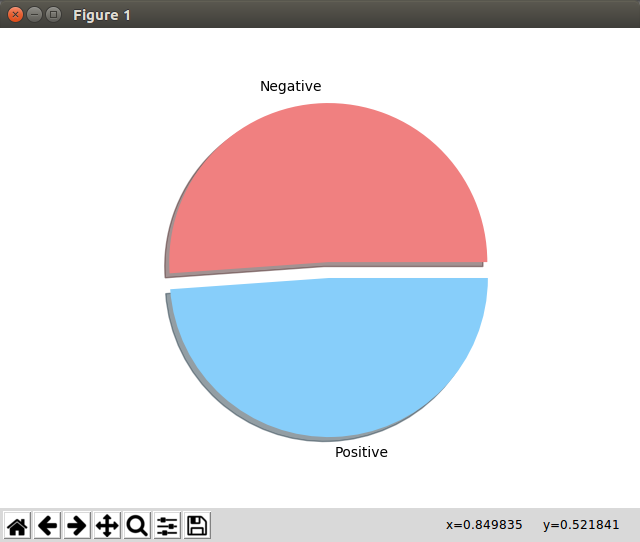
\includegraphics[width=1\linewidth]{5th}
	\caption{Plotting the pie chart from the results}
\end{figure}

In this picture, from the results recieved by the machine, it generates a pie chart for the easy understanding of the user.




\chapter{Conclusion and Future Scope}\hrule
\label{Chapter:6}
% =====================================================================================================
\section{Conclusion}

Sentiment analysis or opinion mining is a field of study that analyzes people’s sentiments, attitudes, or emotions towards certain entities. This paper tackles a fundamental problem of sentiment analysis, sentiment polarity categorization. Online product reviews from Amazon.com are selected as data used for this study. A sentiment polarity categorization process  has been proposed along with detailed descriptions of each step. Experiments for both sentence-level categorization and review-level categorization have been performed.\\

\section{Future Scope}
\begin{itemize}
	\item The project can be made more interactive by developing a beautiful User Interface in Django.
	\item In future, the project can be tailored to satisfy the needs of a particular client by adding the required features or removing the unwanted features.
	\item The project can also be upgraded to a customized algorithm defined by the developer.
	\item The project has a brighter scope and we hope, it will also keep satisfying more and more customers in the future.
\end{itemize}


\chapter{Refrences}\hrule
\label{Chapter:7}
% =====================================================================================================
\begin{enumerate}
	\item Liu B (2010) Sentiment analysis and subjectivity In: Handbook of Natural Language Processing, Second Edition.. Taylor and Francis Group, Boca.[accesed on 24/02/2017].
	\item https://www.tutorialspoint.com/python2.7/ [accesed on 10/03/2017].
	\item Pang B, Lee L (2008) Opinion mining and sentiment analysis. Found Trends Inf Retr2(1-2): 1–135. [accesed daily].
	\item Whitelaw C, Garg N, Argamon S (2005) Using appraisal groups for sentiment analysis  [accesed on \\20/03/2017].
	\item http://textminingonline.com/dive-into-nltk-part-iii-part-of-speech-tagging-and-pos-tagger [accesed on 27/03/2017]
	\item http://textminingonline.com/dive-into-nltk-part-x-play-with-word2vec-models-based-on-nltk-corpus [accesed on 04/04/2017] 

\end{enumerate}